\section{Problem}
Trace the parabola and find its focus.
\begin{align}
144y^2-120xy+25x^2+619x-272y+663=0
\end{align}

\section{Solution}
The general second degree equation can be expressed as follows,
\begin{align}
\Vec{x}^T\Vec{V}\Vec{x}+2\Vec{u}^T\Vec{x}+f=0
\intertext{where,}
\vec{V} &= \myvec{144&-60\\-60&25}\\ \label{eq:conics/ex/solution/given1}
\vec{u} &= \myvec{\cfrac{619}{2}\\-136}\\ 
f &= 663 \label{eq:conics/ex/solution/given2}
\end{align}
\begin{enumerate}
\item Expanding the determinant of $\vec{V}$ we observe, 
\begin{align}
\mydet{144&-60\\-60&25} = 0 \label{eq:conics/ex/solution/eq2.1}
\end{align}
Also
\begin{align}
    \mydet{\vec{V} & \vec{u} \\ \vec{u}^T & f}=
    \mydet{144&-60 & \cfrac{619}{2} \\-60&25 & -136 \\ \cfrac{619}{2} & -136 & 663} \\
    \neq 0\label{eq:conics/ex/solution/eq2.2}
\end{align}
Hence from \eqref{eq:conics/ex/solution/eq2.1} and \eqref{eq:conics/ex/solution/eq2.2} we conclude that given equation is an parabola. The characteristic equation of $\vec{V}$ is given as follows,
\begin{align}
\mydet{\lambda\vec{I}-\vec{V}} = \mydet{\lambda-144&60\\60&\lambda-25} &= 0\\
\implies \lambda^2-169\lambda &= 0\label{eq:conics/ex/solution/eqchar}
\end{align}
Hence the characteristic equation of $\vec{V}$ is given by \eqref{eq:conics/ex/solution/eqchar}. The roots of \eqref{eq:conics/ex/solution/eqchar} i.e the eigenvalues are given by
\begin{align}
\lambda_1=0, \lambda_2=169\label{eq:conics/ex/solution/eqeigenvals}    
\end{align}
\item For $\lambda_1 = 0$, the eigen vector $\vec{p}$ is given by 
\begin{align}
\vec{V}\vec{p} = 0
\end{align}
Row reducing $\vec{V}$ yields
\begin{align}
\implies
\myvec{-144&60\\60&-25}\xleftrightarrow[R_2=R_2+5R_1]{R_1=\frac{R_1}{12}}\myvec{-12&5\\0&0}\\
\implies\vec{p}_1=\cfrac{1}{13}\myvec{5\\12} \label{eq:conics/ex/solution/eq2.3}
\end{align}
Similarly, 
\begin{align}
\vec{p}_2=\frac{1}{13}\myvec{12\\-5} 
\end{align}
%
Thus, the eigenvector rotation matrix and the eigenvalue matrix are
\begin{align}
\vec{P}&=\myvec{\vec{p_1}&\vec{p_2}}=\frac{1}{13}\myvec{5&12\\ 12 &-5} \\
\vec{D}&=\myvec{0&0\\0&169}
\end{align}
The focal length of the parabola is given by 
\begin{align}
\frac{\abs{2\vec{u}^T\vec{p_1}}}{\lambda_2}
    = \frac{13}{169}=\cfrac{1}{13}
\end{align}
and its equation is
\begin{align}
    \vec{y^T}\vec{D}\vec{y}&=-\eta\myvec{1&0}\vec{y}\label{eq:conics/ex/solution/eq2.4}
\end{align}
where
\begin{align}
    \eta=2\vec{u}^T\vec{p_1}=-13
\end{align}
and the vertex $\vec{c}$ is given by 
\begin{align}
    \myvec{\vec{u^T}+\frac{\eta}{2}\vec{p_1^T} \\ \vec{V}}\vec{c}=
    \myvec{-f \\\frac{\eta}{2}\vec{p_1}-\vec{u}} 
\end{align}
using equations \eqref{eq:conics/ex/solution/given1},\eqref{eq:conics/ex/solution/given2} and \eqref{eq:conics/ex/solution/eq2.3}
\begin{align}
    \myvec{307& -142 \\ 144 & -60 \\  -60 & 25 }\vec{c}=\myvec{-663 \\ -312\\ 130} \label{eq:conics/ex/solution/eqcen}
\end{align}
Forming the augmented matrix and row reducing it:
\begin{align}
\myvec{307 & -142 & -663\\144 & -60 & -312 \\-60 & 25 &130 }\\
R_2\leftrightarrow \cfrac{R_2}{12} \nonumber \\
\myvec{307 & -142 & -663\\12 & -5 & -26 \\-60 & 25 &130}\\
R_3\leftrightarrow R_3+5R_2 \nonumber \\
\myvec{307 & -142 & -663\\12 & -5 & -26 \\0 & 0 &0}\\
R_1\leftrightarrow \cfrac{R_1}{307} \nonumber \\
\myvec{1 & \cfrac{-142}{307} & \cfrac{-663}{307}\\0 & \cfrac{169}{307} & \cfrac{-26}{307} \\0 & 0 &0}\\ R_2\leftrightarrow R_2-12R_1 \nonumber \\
\myvec{1 & \cfrac{-142}{307} & \cfrac{-663}{307}\\0 & 1 & \cfrac{-26}{307} \\0 & 0 &0}\\
R_1\leftrightarrow R_1 +(142/307)R_2 \nonumber \\
\myvec{1 & 0 & -29/13\\0 & 1 & -2/13 \\0 & 0 &0}
\end{align}
Thus the vertex $\vec{c}$ is:
\begin{align}
\vec{c}=\myvec{ -29/13\\-2/13} 
\end{align}

The direction vector of axis of symmetry is given by :
\begin{align}
m=Vc+u\\
=\myvec{144&-60\\-60&25}\myvec{-\cfrac{29}{13}\\-\cfrac{2}{13}}+\myvec{\cfrac{619}{2}\\-\cfrac{272}{2}}\\
=\myvec{-\cfrac{5}{2}\\-6}\\
\norm{m}=\cfrac{13}{2}\\
\implies \cfrac{m}{\norm{m}}=\myvec{-\cfrac{5}{13}\\-\cfrac{12}{13}}
\end{align}

The focus is given by:
\begin{align}
F=c-(\cfrac{m}{\norm{m}}\times a)\\
=\myvec{-\cfrac{29}{13}\\-\cfrac{2}{13}}-\myvec{\myvec{-\cfrac{5}{13\\-\cfrac{12}{13}}}\times \cfrac{1}{52}}\\
=\myvec{-\cfrac{1503}{676},-\cfrac{23}{169}}
\end{align}

\begin{figure}[!ht]
    \centering
    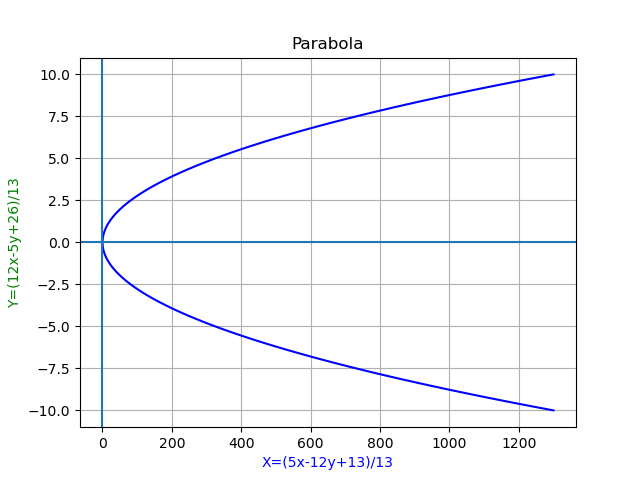
\includegraphics[width=\columnwidth]{./figs/parabola}
\caption{Traced parabola}
\label{parabola}
\end{figure}
\end{enumerate}





